\subsection*{Partie I.}
\begin{enumerate}
 \item \begin{enumerate}
 \item On calcule directement :
\begin{align*}
 &P_0 = 1,\;           T_0= 2 
 &P_1 = X,\;           T_1= X \\
 &P_2 = 2X^2-1,\;      T_2 = X^2 -\frac{1}{2} 
 &P_3 = 4X^3-3X ,\;    T_3 = X^3 -\frac{3}{4}X\\
 &P_4 = 8X^4-8X^2+1,\; T_4 = X^4 -X^2 +\frac{1}{8}
\end{align*}
\item Il est immédiat par récurrence d'après les définitions que $P_n$ et $T_n$ sont de degré $n$ et que $T_n$ est unitaire (coefficient dominant égal à 1).
\item La relation est vraie pour 0 et 1, elle se propage par récurrence car : 
\begin{displaymath}
 \cos ((n+1)\theta) + \cos ((n-1)\theta)= 2\cos \theta \cos (n\theta)
\end{displaymath}
\item Comme $P_n$ est de degré $n$, il admet au plus $n$ racines. Or pour $k$ entre $1$ et $n$ :
\begin{displaymath}
 P_n(x_k)= P_n\left( \cos(\frac{2k-1}{2n}\pi)\right)=\cos\left( n (\frac{2k-1}{2n}\pi)\right) = \cos\left( \frac{2k-1}{2}\pi\right) = 0 
\end{displaymath}
Comme $\frac{2k-1}{2n}\pi \in [0,\pi]$ (intervalle dans lequel la fonction $\cos$ est strictement décroissante) les $x_k$ sont deux à eux distincts. Ils forment donc la famille de \emph{toutes} les racines de $P_n$. Ces racines sont donc simples.

\item Les polynômes $P_n$ et $T_n$ admettent le même ensemble de racines et varient simultanément car ils sont proportionnels (coefficient multiplicatif $2^{n-1}$). La fonction $P_n$ oscille entre $-1$ et $+1$, la fonction $T_n$ entre $-2^{1-n}$ et $+2^{1-n}$.\newline
Dans $[-1,+1]$, la valeur maximale $2^{1-n}$ de $|T_n|$ est atteinte aux points $\cos \theta$ tels que $\cos n\theta = \pm1$ c'est à dire lorsque $n\theta \equiv 0 \mod(\pi)$. La fonction $|T_n|$ atteint donc sa valeur maximale $2^{n-1}$ aux points :
\begin{displaymath}
x_k^\prime = \cos(\frac{k}{\pi}n)\text{ avec } k\in \llbracket 0,n\rrbracket
\end{displaymath}
Comme $\cos$ est strictement décroissant dans $[0,\pi]$, ces $n+1$ points sont bien deux à deux distincts.
%\item Comme les polynômes sont définis par récurrence, il est naturel de proposer une procédure récursive.
%\begin{verbatim}
%cheb := proc(n)
%  if n= 0 then
%    return 1;
%  elif n=1 then
%    return X
%  else
%    return collect(2*X* cheb(n-1) - cheb(n-2),X);
%  fi;
%end proc;
%\end{verbatim} 
%Signalons le \texttt{collect} dans la dernière instruction qui permet de renvoyer le polynôme sous sa forme habituelle en rassemblant les coefficients %des $X^k$. Le nom \texttt{X} ne soit surtout pas être assigné à quoi que ce soit.
\end{enumerate}
\begin{figure}
 \centering
 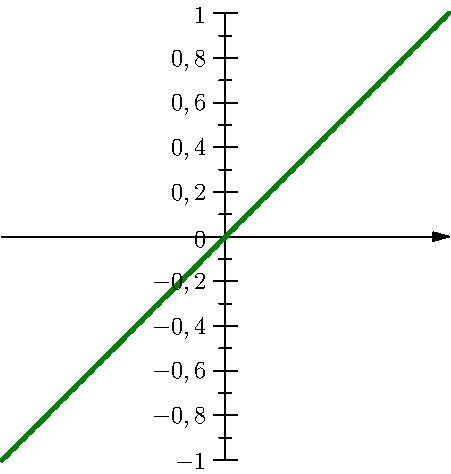
\includegraphics[width=3cm]{Cchebydiam_1.pdf}\hspace{0.2cm}
 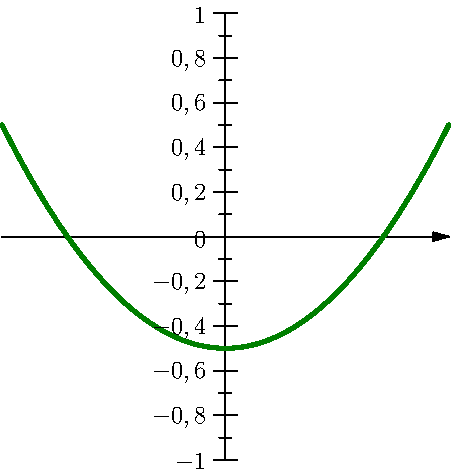
\includegraphics[width=3cm]{Cchebydiam_2.pdf}\hspace{0.2cm}
 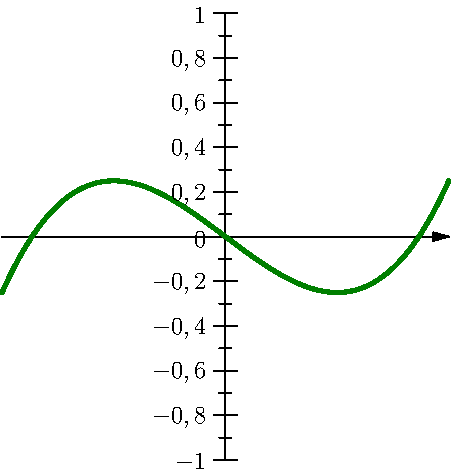
\includegraphics[width=3cm]{Cchebydiam_3.pdf}\hspace{0.2cm}
 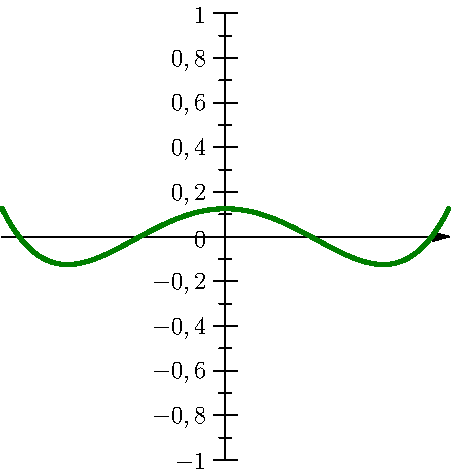
\includegraphics[width=3cm]{Cchebydiam_4.pdf}
 \caption{$T_1, T_2, T_3, T_4$ séparément}
 \label{fig:Cchebydiam_1}
\end{figure}
\begin{figure}
 \centering
 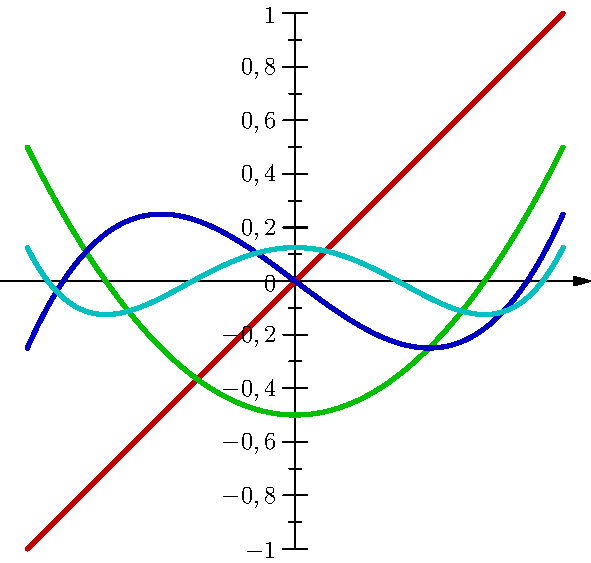
\includegraphics[width=7cm]{Cchebydiam_5.pdf}
 \caption{$T_1, T_2, T_3, T_4$ simultanément}
 \label{fig:Cchebydiam_5}
\end{figure}

\item
\begin{enumerate}
 \item 
 Le tracé des graphes entre $-1$ et $1$ ne pose pas de problème particulier (Fig. \ref{fig:Cchebydiam_1})
Il est intéressant aussi de tracer tous les graphes dans la même figure (Fig. \ref{fig:Cchebydiam_5})
\item Supposons qu'il existe un polynôme unitaire $P$ de degré $n$ tel que
\begin{displaymath}
 \sup_{[0,1]} |P| < 2^{1-n} \Rightarrow \forall x \in [-1, +1] : |P(x)|< 2^{1-n}
\end{displaymath}
Examinons le polynôme $T_n - P$.\newline
Son degré est strictement inférieur à $n$ car $T_n$ et $P$ sont unitaires.\newline
Considérons les $n+1$ points où $T_n$ atteint alternativement $-2^{1-n}$ et $2^{1-n}$. En ces points, le polynôme $T_n -P$ prend alternativement des valeurs strictement négatives et strictement positives. Par continuité $T_n -P$ va donc s'annuler entre deux consécutifs de ces $n+1$ points soit au moins $n$ fois. Comme $\deg (T_n -P) <n$ cela entrainerait $T_n -P=0$ en contradiction avec la condition imposée à $P$.
\item Cette question est une simple reformulation logique de la question précédente.
\item La linéarité et le fait que $(f/f)$ soit positif est facile et classique. Il faut bien prendre garde que c'est la \emph{continuité} de $f^2$ (et sa positivité) qui assure que :
\begin{displaymath}
 (f/f)=0 \Rightarrow f=0
\end{displaymath}
La preuve de l'orthonormalité de la famille vient du calcul des produits scalaires :
\begin{displaymath}
 (P_n/P_m)=\int_0^\pi P_n(\cos\theta) P_m(\cos\theta) d\theta 
 = \int_0^\pi \cos n \theta \cos m\theta  d\theta 
 =  \begin{cases}
     0& \text{si $m=n$}\\ 
     \frac{\pi}{2}& \text{si $m=n$}
    \end{cases}
\end{displaymath}
après linéarisation.
\end{enumerate}
\end{enumerate}

\subsection*{Partie II.}
\begin{enumerate}
 \item \begin{enumerate}
 \item Les nombres $d_2$ et $d_3$ sont bien définis car les ensembles dont ils sont les bornes supérieures sont majorés par $2R$.
\begin{itemize}
 \item Pour tous $A$ et $B$ dans $\Omega$ : 
\begin{displaymath}
 d(A,B)\leq d(A,0)+d(O,B)\leq 2R
\end{displaymath}

 \item Pour tous $A$,  $B$, $C$ dans $\Omega$ : 
\begin{displaymath}
d(A,B,C)=(AB.BC.CA)^{\frac{1}{3}} \leq (2R.2R.2R)^{\frac{1}{3}}\leq 2R 
\end{displaymath}
\end{itemize}

\item Par définition de $d_2$ comme borne supérieure, $AB\leq d_2$ pour tous les points $A$, $B$ de $\Omega$. On en déduit 
\begin{displaymath}
\forall (A,B,C)\in \Omega^3,\; d(A,B,C)=(AB.BC.CA)^{\frac{1}{3}} \leq (d_2.d_2.d_2)^{\frac{1}{3}}\leq d_2 
\end{displaymath}
Cela signifie que $d_2$ est un majorant de l'ensemble dont $d_3$ est la borne supérieure. Par conséquent, comme la borne supérieure d'un ensemble est \emph{le plus petit} des majorants,
\begin{displaymath}
 d_3\leq d_2
\end{displaymath}

\item On raisonne avec deux suite d'implications autour de la définition d'une borne supérieure. Notons
\begin{displaymath}
 \delta = \sup \left\lbrace l(A,B), (A,B)\in \Omega^2 \right\rbrace 
\end{displaymath}
Alors, d'une part :
\begin{multline*}
 \forall A \in \Omega, \forall B \in \Omega, \forall C \in \Omega : d(A,B,C)\leq d_3 \\
\Rightarrow \forall A \in \Omega, \forall B \in \Omega, \left( \forall C \in \Omega : d(A,B,C)\leq d_3 \right) \\
\Rightarrow \forall A \in \Omega, \forall B \in \Omega, l(A,B)\leq d_3
\Rightarrow \delta \leq d_3
\end{multline*}
d'autre part :
\begin{multline*}
 \forall A \in \Omega, \forall B \in \Omega : l(A,B)\leq \delta \\
\Rightarrow \forall A \in \Omega, \forall B \in \Omega, \left( \forall C \in \Omega : d(A,B,C)\leq \delta \right)
\Rightarrow d_3 \leq \delta
\end{multline*}
\end{enumerate}

\item Lorsque $\Omega$ est un segment de longueur $a$, il est clair que $d_2=a$.\newline
Il est naturel de considérer la configuration particulière où $A$ et $B$ sont les deux extrémités du segment et $C$ le milieu. Pour cette configuration :
\begin{displaymath}
 d(A,B,C) = \left( a(\frac{a}{2})^2\right) ^{\frac{1}{3}} = a\,4^{-\frac{1}{3}} \Rightarrow d_3 \geq a\,4^{-\frac{1}{3}}
\end{displaymath}
Pour une configuration quelconque, remarquons d'abord que l'ordre des points $A$, $B$, $C$ est sans importance. On supposera donc $C$ entre $A$ et $B$ avec de plus $AC = x AB$, $BC=(1-x)AB$ pour $x\in[0,1]$. Avec ces notations :
\begin{displaymath}
 d(A,B,C)=(x(1-x))^{\frac{1}{3}}AB
\end{displaymath}
L'étude de la fonction $x\rightarrow (x(1-x))^{\frac{1}{3}}$ montre rapidement qu'elle atteint son maximum absolu en $\frac{1}{2}$. Le plus grand des $d(A,B,C)$ est donc atteint lorsque $C$ est au milieu de $A$ et $B$ et que $AB$ est le plus grand possible On retrouve la configuration du début et on a prouvé que
\begin{displaymath}
 d_3 = a\,4^{-\frac{1}{3}}
\end{displaymath}
On peut remarquer que ce raisonnement rend inutile la considération de la configuration particulière.
\item 
\begin{figure}
   \centering
   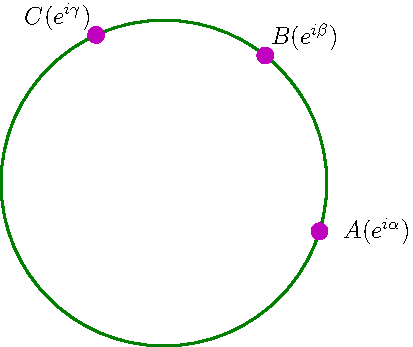
\includegraphics[width=3cm]{Cchebydiam_6.pdf}
   \caption{II.3.d Calcul de $d_3$ pour un cercle}
   \label{fig:Cchebydiam_6}
\end{figure}

\begin{enumerate}
 \item Le calcul suivant est plus que classique :
 \begin{displaymath}
 Re^{i\beta} - R e^{i\alpha} = Re^{i\frac{\alpha + \beta}{2}}
\left( e^{i\frac{-\alpha + \beta}{2}} - e^{i\frac{\alpha - \beta}{2}}\right)  = 
2iR\sin\frac{\beta -\alpha}{2}e^{i\frac{\alpha + \beta}{2}}
\end{displaymath}
Lorsque $A$ et $B$ sont respectivement les points d'affixes $Re^{i\alpha}$ et $Re^{i\beta}$, la distance $AB$ est le module du complexe du dessus. Soit :
\begin{displaymath}
 AB = 2R\sin\frac{\beta -\alpha}{2}
\end{displaymath}
Dans la configuration indiquée par l'énoncé ($\sin$ positif).
\item La dérivée en $\beta$ de la fonction indiquée par l'énoncé est :
\begin{displaymath}
 \frac{1}{2}\sin\left( \frac{\alpha + \gamma}{2}-\beta\right) 
\end{displaymath}
Dans le domaine indiqué par l'énoncé (Fig. \ref{fig:Cchebydiam_6}), cette fonction admet bien son maximum en $\frac{\alpha + \gamma}{2}$. La valeur maximale est 
\begin{displaymath}
  \sin^2 \frac{\gamma - \alpha}{4}
\end{displaymath}

\item Le calcul de la dérivée de la fonction $\varphi$ de l'énoncé conduit à :
\begin{displaymath}
 \varphi^\prime(t)=\frac{t^2}{\sqrt{1-t^2}}(3-4t^2)
\end{displaymath}
On en déduit le tableau de variations:
\begin{displaymath}
\renewcommand{\arraystretch}{1.4}
 \begin{array}{|ccccc|}
  \hline
 0 & & \frac{\sqrt{3}}{2}   &          & 1 \\ \hline
   & & \frac{3\sqrt{3}}{16} &          &  \\
   & \nearrow &              & \searrow &  \\
 0 & &  & & 0 \\ \hline
\end{array}
\end{displaymath}
\item La configuration de la figure (Fig. \ref{fig:Cchebydiam_6}) est la plus générale (après une éventuelle permutation des points sans conséquence sur la distance. Dans ces conditions (en majorant par 3.b.):
\begin{multline*}
 AB.AC.BC = (2R)^3 \left( \sin\frac{\beta - \alpha}{2} \sin\frac{\gamma - \beta}{2}\right)  \sin\frac{\gamma - \alpha}{2} \\
\leq (2R)^3 \sin^2 \frac{\gamma - \alpha}{4} \sin\frac{\gamma - \alpha}{2}
= (2R)^3\, 2 \sin^3 \frac{\gamma - \alpha}{4} \cos \frac{\gamma - \alpha}{4} \\
= 16 R^3\, \varphi(\sin \frac{\gamma - \alpha}{4}) \leq 16 R^3\, \frac{3\sqrt{3}}{16}
= (\sqrt{3} R)^3
\end{multline*}
On en déduit $d_3\leq \sqrt{3}R$. Pour montrer l'égalité, on vérifie que cette valeur est atteinte lorsque le triangle $(A,B,C)$ est équilatéral.
\end{enumerate}
\end{enumerate}

\subsection*{Partie III.}
\begin{enumerate}
 \item
\begin{enumerate}
 \item On admet que $(\lambda_1,\cdots,\lambda_{n+1})$ réalise la borne supérieure $D_{n+1}$. Dans l'expression de $D_{n+1}$ on sépare alors les facteurs contenant $\lambda_1$ de ceux qui ne le contiennent pas, puis on majore.
\begin{multline*}
 D_{n+1}=(\lambda_2-\lambda_1)\cdots(\lambda_{n+1}-\lambda_1)D(\lambda_2,\cdots,\lambda_{n+1})\\
\leq |\lambda_2-\lambda_1|\cdots |\lambda_{n+1}-\lambda_1| \sup\left\lbrace D(\mu_1,\cdots,\mu_n),(\mu_1,\cdots,\mu_n)\in\R^n\right\rbrace \\
\leq |\lambda_2-\lambda_1|\cdots |\lambda_{n+1}-\lambda_1| D_n
\end{multline*}
\item On peut écrire des inégalités analogues à la précédente en faisant varier l'indice du $\lambda$ jouant un rôle particulier (valeur 1) dans la majoration précédente.
\begin{displaymath}
\left. 
\begin{aligned}
 D_{n+1} \leq& D_n \prod_{i\neq 1}|\lambda_i-\lambda_1| \\
 D_{n+1} \leq& D_n \prod_{i\neq 2}|\lambda_i-\lambda_2| \\
 \vdots& \\
 D_{n+1} \leq& D_n \prod_{i\neq n+1}|\lambda_i-\lambda_{n+1}|  
\end{aligned}
\right\rbrace \Rightarrow
D_{n+1}^{n+1} \leq D_{n}^{n+1}D_{n+1}^{2}  \text{ (en faisant le produit)}
\end{displaymath}
Le carré vient de ce que, dans $D_{n+1}$, on impose $i<j$. En simplifiant:
\begin{displaymath}
 D_{n+1}^{n-1} \leq D_{n}^{n+1}
\end{displaymath}
\item On va montrer que $(d_n)_{n\in\N}$ est décroissante. On exprime les $D$ en fonction des $d$ :
\begin{displaymath}
 D_n=d_n^{\frac{n(n-1)}{2}}, \hspace{0.5cm}
D_{n+1}=d_{n+1}^{\frac{n(n+1)}{2}}
\end{displaymath}
Puis on remplace dans l'inégalité de la question précédente qui devient:
\begin{displaymath}
 d_{n+1}^{\frac{n(n+1)(n-1)}{2}} = D_{n+1}^{n-1}  \leq D_{n}^{n+1} = d_n^{\frac{n(n-1)(n+1)}{2}}
\end{displaymath}
Cela conduit à $d_{n+1}\leq d_n$ car les exposants sont identiques. La suite est positive et décroissante donc convergente. Soit $d$ sa limite.
\end{enumerate}
\item 
\begin{enumerate}
 \item D'après I.2.c. :
\begin{displaymath}
 \mu_n = 2^{1-n}, \hspace{0.5cm} m_n = 2^{\frac{1-n}{n}}=2^{-1+\frac{1}{n}}
\end{displaymath}
\item D'après l'expression du dessus, $(m_n)_{n\in\N^*}$ converge clairement vers $\frac{1}{2}$.
\item Il s'agit d'une variante du théorème de Césaro qui se démontre de la même manière.
\end{enumerate}
 
\item 
\begin{enumerate}
 \item En ajoutant dans la dernière ligne du déterminant (celui qui figure à droite de la relation demandée) une combinaison linéaire des autres lignes, on ne modifie pas sa valeur mais on peut faire disparaitre tous les termes de $P$ sauf celui de degré $n$. On obtient donc $V_n(x_1,\cdots,x_n)$.
\item Notons $V_i$ le déterminant $n\times n$ de VanderMonde formé à partir de $V(x_1,\cdots,x_{n+1})$ en supprimant $x_i$ de la famille. Il est aussi obtenu en supprimant la dernière ligne et la colonne des $x_i$ du déterminant de 3.a Le développement de l'expression de $V(x_1,\cdots,x_{n+1})$ trouvée à la question précédente le long de la dernière ligne puis des majorations utilisant les définitions conduisent à :
\begin{multline*}
 V(x_1,\cdots,x_{n+1}) = \sum_{i=1}^{n} (-1)^{n+i}V_i \\
 \Rightarrow
|V(x_1,\cdots,x_{n+1})| \leq (n+1) D_n \mu_n \Rightarrow
D_{n+1} \leq D_n \mu_n
\end{multline*}
car chaque déterminant est en valeur absolue majoré par $D_n$ et chaque valeur du polynôme par $\mu_n$. Puis, comme 
\begin{displaymath}
 D_n = d_n^{\frac{n(n-1)}{2}}, \hspace{0.5cm}  D_{n+1} = d_{n+1}^{\frac{n(n+1)}{2}}, \hspace{0.5cm} \mu_n = m_n^n
\end{displaymath}
On déduit la relation demandée :
\begin{displaymath}
 d_{n+1}^{\frac{n(n+1)}{2}} \leq (n+1)d_n^{\frac{n(n-1)}{2}}m_n^n
\end{displaymath}
\item On sépare dans $V(x_1,\cdots,x_{n+1})$ les facteurs commençant par $x_{n+1}$ :
\begin{multline*}
 V(x_1,\cdots,x_{n+1})=(x_{n+1}-x_1)\cdots(x_{n+1}-x_n)V(x_1,\cdots,x_n)\\
=P(x_{n+1})V(x_1,\cdots,x_n)
\end{multline*}
Comme ceci est valable pour toutes les familles $(x_1,\cdots,x_{n+1})$, on en tire :
\begin{displaymath}
 |P(x_{n+1})||V(x_1,\cdots,x_n)| \leq D_{n+1} \text{ et }
 |V(x_1,\cdots,x_n)| \leq \frac{D_{n+1}}{ |P(x_{n+1})|}
\leq \frac{D_{n+1}}{ \mu_n}
\end{displaymath}
car $|P(x_{n+1})|\geq \mu_n$. Par définition d'une borne supérieure: :
\begin{displaymath}
 D_n \leq \frac{D_{n+1}}{ \mu_n} 
 \Rightarrow
 m_n^n\, d_n^{\frac{n(n-1)}{2}} \leq d_{n+1}^{\frac{n(n+1)}{2}}
\end{displaymath}

\item On fait apparaitre un quotient dans l'inégalité précédente :
\begin{displaymath}
 m_n d_n^{\frac{n-1}{2}}\leq d_{n+1}^{\frac{n+1}{2}}
\Rightarrow m_n \leq d_{n+1}\frac{d_{n-1}^{\frac{n+1}{2}}}{d_{n}^{\frac{n+1}{2}}}
= d_{n+1}\left(\frac{d_{n-1}}{d_n} \right)^{\frac{n+1}{2}} \leq d_{n+1}
\end{displaymath}
Le dernier quotient est $\leq 1$ car la suite $d_n$ est décroissante. 
\item Comme les suites sont convergentes, on  obtient, par passage à la limite dans l'inégalité précédente,
\begin{displaymath}
 \frac{1}{2}=m\leq d
\end{displaymath}
L'inégalité de la question 3.b. fait intervenir des termes consécutifs d'une suite $\frac{k(k-1)}{2}d_k$. En prenant le $\ln$, on peut sommer en domino. 
\begin{displaymath}
 \frac{k(k+1)}{2} \ln(d_{k+1}) \leq \frac{(k-1)k}{2} \ln(d_{k}) + \ln(k) + k\ln(m_k) 
\end{displaymath}
pour $k$ entre $1$ et $n$:
\begin{displaymath}
  \frac{n(n+1)}{2}\ln(d_{n+1}) \leq  \sum_{k=1}^n\ln(k) + \sum_{k=1}^nk\ln(m_k)
\end{displaymath}
De plus,
\begin{displaymath}
  \sum_{k=1}^n\ln(k) \leq n\ln(n) \Rightarrow \frac{\sum_{k=1}^n\ln(k)}{n(n+1)} \rightarrow 0, \hspace{0.5cm}
    \frac{\sum_{k=1}^nk\ln(m_k)}{\frac{n(n+1)}{2}} \rightarrow \ln(m)
\end{displaymath}
d'après la question 2.c. Par passage à la limite dans une inégalité:
\begin{displaymath}
  \ln(d) \leq \ln(m)\Rightarrow d \leq \frac{1}{2}
\end{displaymath}

\end{enumerate}
\end{enumerate}
